\documentclass[conference]{IEEEtran}
\IEEEoverridecommandlockouts
\usepackage[numbers]{natbib}
\usepackage{graphicx}
\usepackage{amsmath,amssymb,amsfonts}
\usepackage{hyperref}
\usepackage{caption}
\usepackage{subcaption}
\usepackage{booktabs}
\usepackage{siunitx}
\usepackage{float}
\usepackage{listings}

\lstset{
  basicstyle=\footnotesize\ttfamily,
  breaklines=true,
  frame=single,
  numbers=left,
  numberstyle=\tiny,
  xleftmargin=2em,
  columns=flexible
}

% Reduce spacing around figures
\captionsetup[figure]{skip=2pt}
\setlength{\textfloatsep}{5pt}
\setlength{\intextsep}{5pt}

\title{A Deep Learning Pipeline for Automated News Clustering and Retrieval: Methods, Challenges, and Solutions}

\author{
\IEEEauthorblockN{Varun Dogra}
\IEEEauthorblockA{
Associate Professor, School of Computer Science \\
and Engineering, Lovely Professional University \\
Phagwara, Punjab 144411, India \\
dogra\_varun@yahoo.com
}
\and
\IEEEauthorblockN{Ayan Ruzdan}
\IEEEauthorblockA{
Student, School of Computer Science \\
and Engineering, Lovely Professional University \\
Phagwara, Punjab 144411, India \\
ayanruzdan@gmail.com
}
}

\begin{document}
\maketitle

\begin{abstract}
    This paper presents a deep learning pipeline for automated news clustering and retrieval, addressing the challenge of organizing and accessing large-scale news archives. The system employs web scraping, semantic clustering with SentenceTransformer embeddings and K-means, and probabilistic topic modeling with Latent Dirichlet Allocation (LDA) to group science news articles by topic, followed by keyword extraction and temporal trend visualization. A Retrieval-Augmented Generation (RAG) chatbot enables conversational querying. Challenges include noisy data, optimal cluster/topic selection, and computational efficiency. Solutions involve robust preprocessing, elbow method optimization for K-means, preset topic counts for LDA, and modular design. The pipeline supports applications in journalism and research, offering scalable insights into news content.
\end{abstract}

\begin{IEEEkeywords}
    clustering, deep learning, news retrieval, SentenceTransformers, K-means, Latent Dirichlet Allocation, Retrieval-Augmented Generation, visualization, Streamlit
\end{IEEEkeywords}

\section{Introduction}
The rapid growth of textual data on digital platforms has heightened the need for intelligent systems to extract structured insights from unstructured news articles \cite{hotho2005brief}. News clustering and retrieval are critical tasks in Natural Language Processing (NLP), enabling machines to organize articles by topic and deliver context-aware responses to user queries \cite{manning2008introduction}. By identifying ``what happened, when, and where,'' these systems support applications such as information retrieval, trend analysis, and policy monitoring \cite{blei2003latent}. This paper presents a deep learning pipeline that integrates web scraping, semantic clustering with K-means, probabilistic topic modeling with Latent Dirichlet Allocation (LDA), temporal trend analysis, and conversational retrieval to manage information overload in science news archives, focusing on methods, challenges, and solutions.

\section{System Architecture}
The pipeline processes science news articles, relevant to fields like journalism and academic research, to track trends and enable informed decision-making. The architecture combines web scraping, semantic clustering with K-means, topic modeling with LDA, visualization, and Retrieval-Augmented Generation (RAG) to structure and access news content, addressing challenges such as noisy data and computational scalability \cite{allahyari2017text}.

\subsection{Web Scraping}
A two-stage scraper extracts metadata (title, URL) and full content (date, body) from science news websites, storing data in JSONL format for efficient processing \cite{mitchell2018web}.

\subsection{Data Preprocessing and Embedding}
Text is preprocessed by removing stopwords and news-specific terms (e.g., ``said'') \cite{jurafsky2009speech}. The all-MiniLM-L12-v2 SentenceTransformer model generates 384-dimensional embeddings for K-means clustering, stored in a FAISS vector store for efficient retrieval \cite{johnson2019billion}. For LDA, texts are tokenized and filtered to create a document-term matrix using CountVectorizer.

\subsection{Clustering and Topic Modeling}
K-means clusters SentenceTransformer embeddings, with the elbow method determining the optimal number of clusters (e.g., 5) \cite{hartigan1979algorithm}. LDA, a probabilistic model, identifies topics by modeling word co-occurrences, using a preset number of topics (e.g., 5) \cite{blei2003latent}. Frequency-based keyword extraction assigns the top 5 keywords to clusters and topics for interpretability \cite{grootendorst2020keybert}.

\subsection{Visualization}
Principal Component Analysis (PCA) projects embeddings to 2D for scatter plots, displayed via Streamlit \cite{van2008visualizing,streamlit2020}. Temporal trend plots illustrate cluster and topic frequencies over time \cite{wei2010lda}. Word clouds visualize LDA topic keywords to highlight thematic content.

\subsection{Conversational Retrieval}
A RAG chatbot, leveraging SerpAPI, FAISS, and Gemini Pro, provides context-aware responses through a Streamlit interface, enabling interactive querying of the news archive \cite{lewis2020retrieval,radford2019language}.

\subsection{Extensibility}
The modular design supports alternative models (e.g., BERT variants, multilingual LDA) and scalable processing, facilitating adaptation to diverse datasets and languages \cite{devlin2019bert}.

\section{Literature Review}
News clustering groups articles by topical similarity, a task rooted in text mining and NLP \cite{hotho2005brief}. Traditional methods like Latent Dirichlet Allocation (LDA) \cite{blei2003latent} use probabilistic modeling to uncover latent topics but face challenges with dynamic news streams \cite{hoffman2010online}. Deep learning approaches, such as Sentence-BERT \cite{reimers2019sentencebert}, produce dense embeddings for clustering, with models like all-MiniLM-L12-v2 balancing efficiency and performance \cite{wang2020minilm}. K-means clustering is simple but may yield less interpretable results compared to LDA’s probabilistic topics \cite{blei2003latent,hartigan1979algorithm}. Clustering evaluation metrics, such as silhouette score and Davies-Bouldin index, quantify cluster quality \cite{rousseeuw1987silhouettes,davies1979cluster}. Keyword extraction methods, such as KeyBERT \cite{grootendorst2020keybert}, improve topic interpretability. Visualization techniques like PCA \cite{van2008visualizing} and interactive platforms like Streamlit \cite{streamlit2020} enhance user engagement. Temporal trend analysis of topics has been explored with LDA to track evolving themes \cite{wei2010lda}. Web scraping frameworks enable large-scale data collection but require robust handling of noisy data \cite{mitchell2018web}. Efficient indexing with FAISS supports scalable retrieval \cite{johnson2019billion}. Retrieval-Augmented Generation \cite{lewis2020retrieval} and advances in conversational AI \cite{radford2019language} improve query accuracy, distinguishing our system from static clustering approaches. Preprocessing techniques, including stopword removal and tokenization, are critical for text analysis \cite{jurafsky2009speech}. Multilingual models like BERT variants offer extensibility for diverse datasets \cite{devlin2019bert}. These works collectively inform our pipeline’s design, addressing challenges in clustering, retrieval, and scalability.

\section{Implementation}
The pipeline, implemented in Python, integrates web scraping, clustering, topic modeling, visualization, and retrieval. Below is pseudocode formatted for clarity and readability.

\subsection{Web Scraping}
\begin{lstlisting}
function scrape_metadata(base_url, max_pages):
    articles = []
    for page in 1 to max_pages:
        html = fetch_webpage(base_url + page)
        parse html to find article cards
        for each card:
            extract title, url
            articles.append({title, url})
    save articles to JSON file
    return articles

function scrape_content(articles):
    results = []
    for article in articles:
        html = fetch_webpage(article.url)
        parse html to extract date, body
        if date and body exist:
            results.append({title, url, date, body})
    save results to JSONL file
\end{lstlisting}

\subsection{Clustering and Topic Modeling}
\begin{lstlisting}
function cluster_articles(articles, num_clusters):
    texts = extract_text(articles)
    embeddings = encode_texts(texts, SentenceTransformer)
    kmeans = apply_kmeans(embeddings, num_clusters)
    labels = kmeans.labels
    keywords = extract_keywords(texts, labels)
    pca = reduce_dimensions(embeddings, 2)
    plot_scatter(pca, labels, keywords)
    save_assignments(articles, labels, keywords, CSV)
    return labels, keywords

function perform_lda(articles, num_topics):
    texts = extract_text(articles)
    doc_term_matrix = vectorize_texts(texts, CountVectorizer)
    lda = apply_lda(doc_term_matrix, num_topics)
    topic_words = extract_top_words(lda, vectorizer)
    assignments = assign_topics(texts, lda, vectorizer)
    save_results(articles, assignments, topic_words, CSV)
    plot_wordclouds(topic_words)
    return assignments, topic_words

function extract_keywords(texts, labels):
    for each cluster in unique(labels):
        cluster_texts = texts where label equals cluster
        words = tokenize_and_filter(cluster_texts)
        top_keywords = most_frequent(words, 5)
        keywords[cluster] = top_keywords
    return keywords

function extract_top_words(lda, vectorizer):
    for each topic in lda.components:
        top_indices = sort_topic_words(topic, descending)
        top_words = get_feature_names(vectorizer, top_indices, 5)
        topic_words[topic] = top_words
    return topic_words
\end{lstlisting}

\subsection{Temporal Trend Analysis}
\begin{lstlisting}
function analyze_temporal_trends(cluster_data, topic_data):
    load cluster assignments from CSV
    load topic assignments from CSV
    convert dates to datetime
    group clusters by date to count articles
    group topics by date to count articles
    plot line graph of cluster counts over time
    plot line graph of topic counts over time
    for each cluster/topic:
        group keywords by date
        count top keywords
        plot line graph of keyword frequencies
    save plots as PNG
\end{lstlisting}

\subsection{Conversational RAG Interface}
\begin{lstlisting}
function handle_query(user_query):
    search_results = search_web(user_query, SerpAPI)
    context = combine_titles_and_snippets(search_results)
    prompt = build_prompt(user_query, context, chat_history)
    response = generate_response(prompt, Gemini)
    display_response(response)
    update_chat_history(user_query, response)
\end{lstlisting}

\section{Figures and Tables}\label{sec:figures-tables}
\begin{figure}[t]
    \centering
    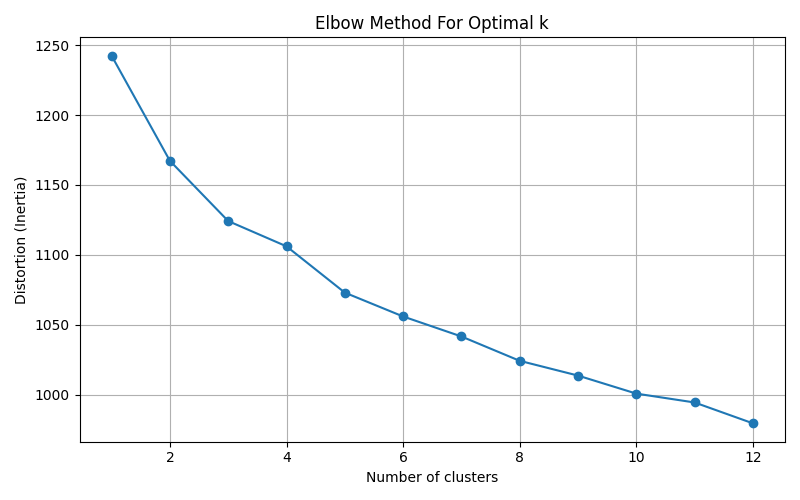
\includegraphics[width=0.45\textwidth]{elbow_plot.png}
    \caption{Elbow plot for determining the optimal number of clusters in K-means.}
    \label{fig:elbow-plot}
\end{figure}

\begin{figure}[t]
    \centering
    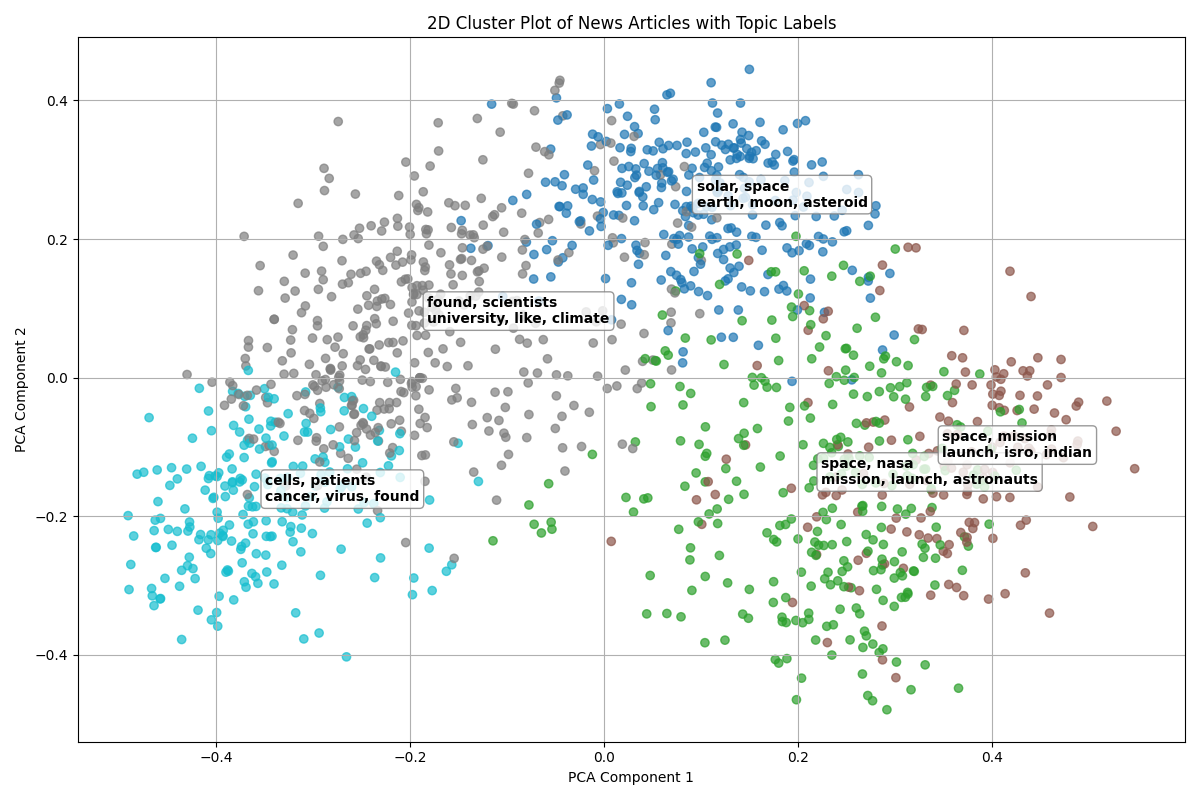
\includegraphics[width=0.45\textwidth]{cluster_plot.png}
    \caption{2D visualization of K-means cluster assignments using PCA.}
    \label{fig:cluster-plot}
\end{figure}

\begin{figure}[t]
    \centering
    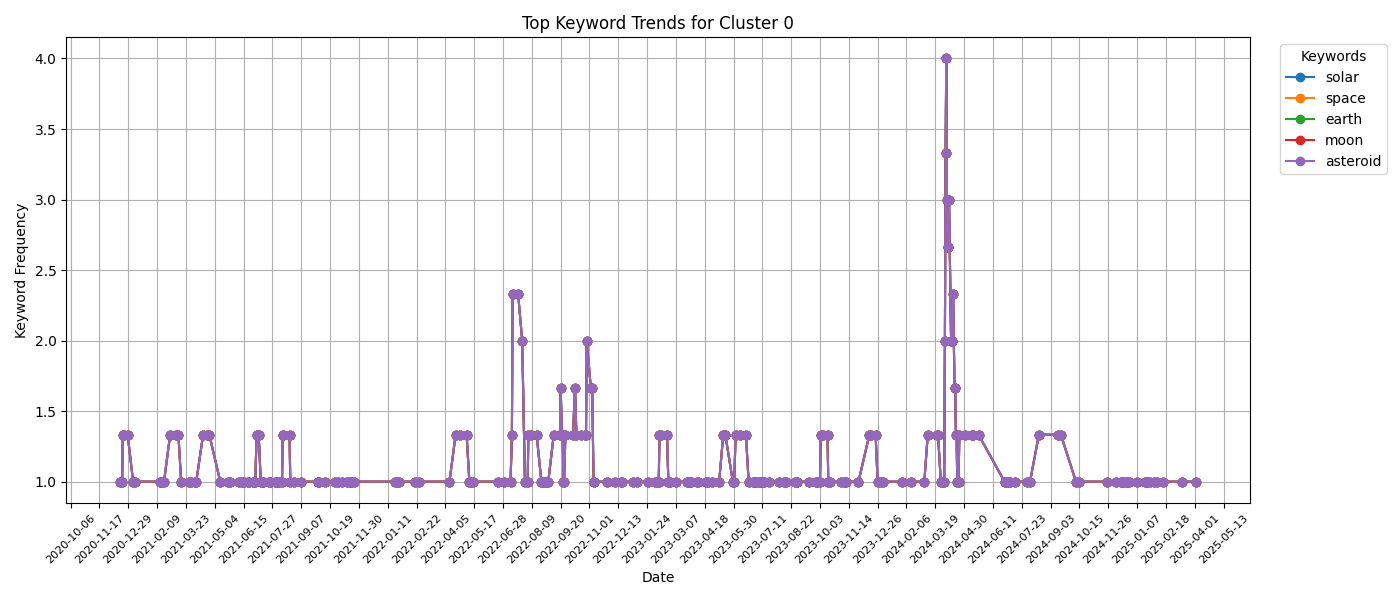
\includegraphics[width=0.45\textwidth]{cluster_0_keywords.png}
    \caption{Top keywords from K-means Cluster 0.}
    \label{fig:cluster0-keywords}
\end{figure}

\begin{figure}[t]
    \centering
    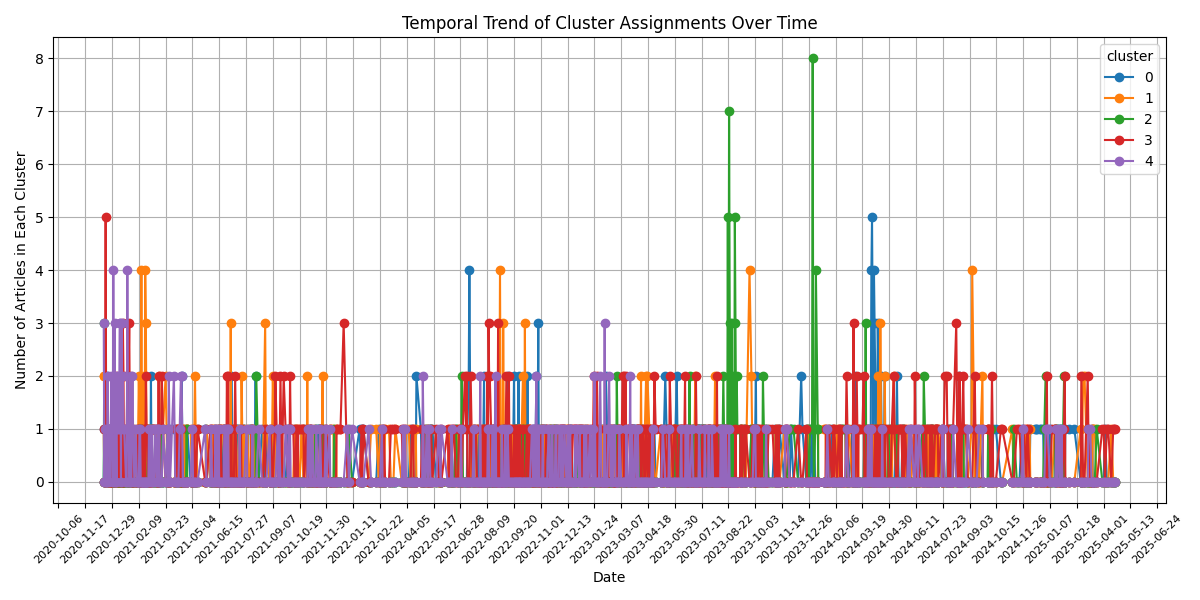
\includegraphics[width=0.45\textwidth]{cluster_trends_over_time.png}
    \caption{Temporal trend of K-means cluster assignments, showing article counts per cluster over time.}
    \label{fig:cluster-trends}
\end{figure}

\begin{figure}[t]
    \centering
    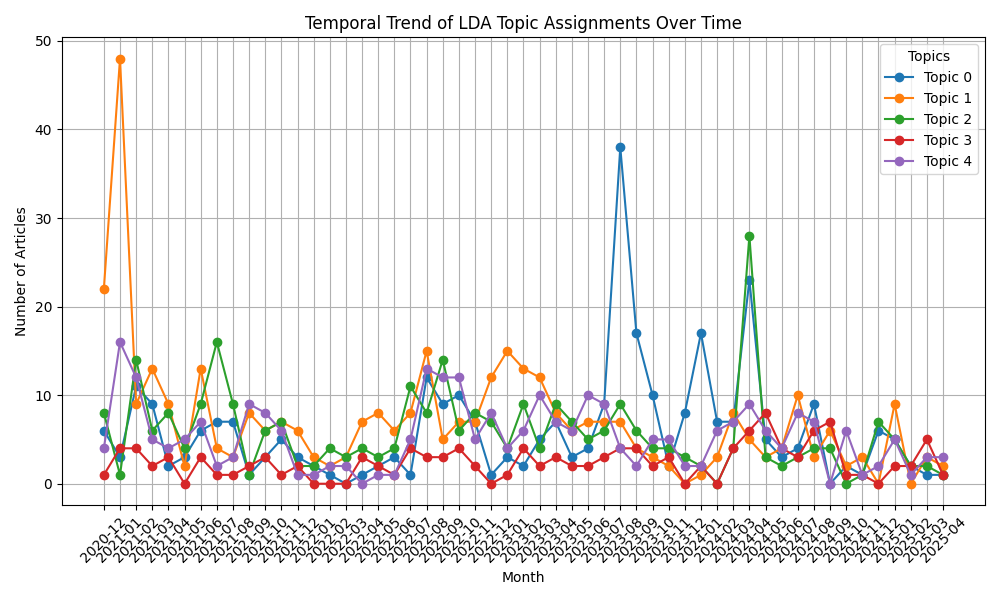
\includegraphics[width=0.45\textwidth]{topic_trends_over_time.png}
    \caption{Temporal trend of LDA topic assignments, showing article counts per topic over time.}
    \label{fig:topic-trends}
\end{figure}

\begin{figure}[t]
    \centering
    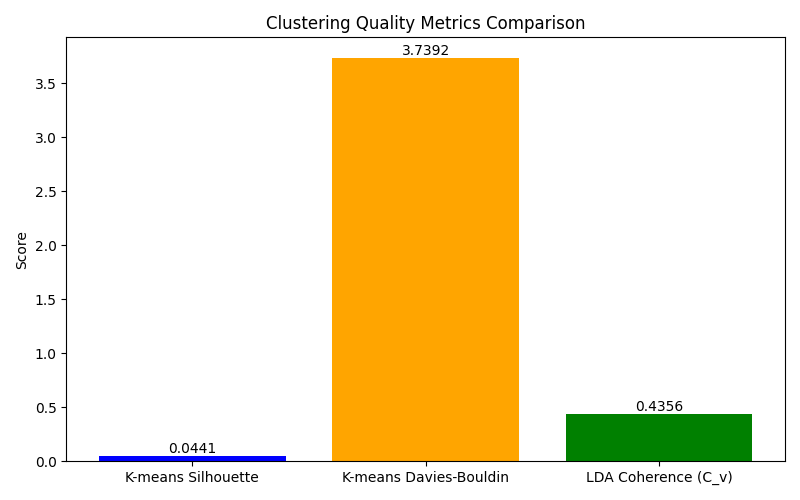
\includegraphics[width=0.45\textwidth]{metrics_comparison.png}
    \caption{Comparison of K-means and LDA clustering quality metrics.}
    \label{fig:metrics-comparison}
\end{figure}

\begin{table}[H]
    \centering
    \caption{Performance Metrics of K-means for News Clustering}
    \label{tab:kmeans_metrics}
    \renewcommand{\arraystretch}{1.4}
    \resizebox{\columnwidth}{!}{%
        \begin{tabular}{|l|c|p{6.5cm}|}
            \hline
            \textbf{Metric}           & \textbf{Value}         & \textbf{Description}                                                                                     \\
            \hline
            Number of Articles        & 1440                   & Total articles processed for clustering.                                                                 \\
            Number of Clusters        & 5                      & Clusters determined via elbow method.                                                                    \\
            Silhouette Score          & 0.04                   & Measures cluster cohesion and separation (range: $[-1, 1]$, higher is better).                           \\
            Davies-Bouldin Index      & 3.74                   & Measures cluster compactness and separation (lower is better).                                           \\
            Distribution Entropy      & 1.92                   & Shannon entropy of cluster distribution (higher is more balanced, max $\approx \log_2(5) \approx 2.32$). \\
            Keyword Overlap (Jaccard) & 0.14                   & Average Jaccard similarity between K-means and LDA keywords (range: $[0, 1]$, lower is more distinct).   \\
            Avg Cosine Similarity     & 0.51                   & Average cosine similarity within clusters (range: $[0, 1]$, higher is tighter).                          \\
            Clustering Time           & $\sim\SI{12}{\second}$ & Time for K-means clustering.                                                                             \\
            \hline
        \end{tabular}%
    }
\end{table}

\begin{table}[H]
    \centering
    \caption{Performance Metrics of LDA for News Clustering}
    \label{tab:lda_metrics}
    \renewcommand{\arraystretch}{1.4}
    \resizebox{\columnwidth}{!}{%
        \begin{tabular}{|l|c|p{6.5cm}|}
            \hline
            \textbf{Metric}           & \textbf{Value}           & \textbf{Description}                                                                                   \\
            \hline
            Number of Articles        & 1440                     & Total articles processed for topic modeling.                                                           \\
            Number of Topics          & 5                        & Topics preset for LDA modeling.                                                                        \\
            Topic Coherence ($C_v$)   & 0.44                     & Measures semantic coherence of topics (range: $[0, 1]$, higher is better).                             \\
            Distribution Entropy      & 2.15                     & Shannon entropy of topic distribution (higher is more balanced, max $\approx \log_2(5) \approx 2.32$). \\
            Keyword Overlap (Jaccard) & 0.14                     & Average Jaccard similarity between K-means and LDA keywords (range: $[0, 1]$, lower is more distinct). \\
            Avg Cosine Similarity     & 0.60                     & Average cosine similarity within topics (range: $[0, 1]$, higher is tighter).                          \\
            Vectorization Time        & $\sim\SI{10.5}{\second}$ & Time for CountVectorizer on CPU.                                                                       \\
            Topic Modeling Time       & $\sim\SI{15.8}{\second}$ & Time for LDA topic modeling on CPU.                                                                    \\
            \hline
        \end{tabular}%
    }
\end{table}

\section{Results and Discussion}
The system was tested on a dataset of 1440 science news articles, with K-means clustering guided by the elbow method (Fig. \ref{fig:elbow-plot}) and LDA using a preset number of topics (5). Due to computational constraints, keyword examples are drawn from a subset of the data, with K-means clusters including:
\begin{itemize}
    \item \textbf{Cluster 0}: cell, patient, cancer, virus, found
    \item \textbf{Cluster 1}: found, science, university, like, climate
    \item \textbf{Cluster 2}: solar, space, earth, moon, asteroid
    \item \textbf{Cluster 3}: space, mission, launch, isro, indian
    \item \textbf{Cluster 4}: space, nasa, mission, launch, astronauts
\end{itemize}
LDA topics from the subset include:
\begin{itemize}
    \item \textbf{Topic 0}: space, mission, lunar, isro, solar
    \item \textbf{Topic 1}: cells, brain, covid, species, human
    \item \textbf{Topic 2}: earth, nasa, space, moon, planet
    \item \textbf{Topic 3}: space, nasa, station, crew, astronauts
    \item \textbf{Topic 4}: water, scientists, cancer, life, earth
\end{itemize}
Performance metrics for K-means and LDA are summarized in Tables \ref{tab:kmeans_metrics} and \ref{tab:lda_metrics}. K-means exhibits a low silhouette score ($0.04$) and high Davies-Bouldin index ($3.74$), suggesting limited cluster separation, possibly due to overlapping themes in science news \cite{rousseeuw1987silhouettes,davies1979cluster}. LDA achieves a moderate topic coherence ($C_v = 0.44$), indicating more interpretable topics \cite{roder2015exploring}. LDA’s higher distribution entropy ($2.15$ vs. $1.92$) reflects a more balanced topic distribution, and its higher average cosine similarity ($0.60$ vs. $0.51$) suggests greater topic cohesion. The low Jaccard similarity ($0.14$) between K-means and LDA keywords underscores their complementary thematic capture \cite{jaccard1912distribution}.

PCA visualization (Fig. \ref{fig:cluster-plot}) illustrates K-means cluster distributions, with keyword plots (Fig. \ref{fig:cluster0-keywords}) highlighting topical focus. Temporal trend analysis (Figs. \ref{fig:cluster-trends}, \ref{fig:topic-trends}) reveals patterns in cluster and topic prevalence, with LDA showing more balanced distributions over time \cite{wei2010lda}. The metrics comparison (Fig. \ref{fig:metrics-comparison}) highlights LDA’s superior coherence and faster processing (total: $\sim\SI{26.3}{\second}$ vs. K-means’ $\sim\SI{444}{\second}$, including embedding time).

The RAG chatbot, accessed via Streamlit, effectively handles queries like ``What AI advancements occurred in 2024?'' by leveraging cluster and topic assignments \cite{radford2019language}. Challenges include noisy web-scraped data, optimal cluster/topic selection, and computational demands \cite{allahyari2017text}. Solutions involve robust preprocessing (e.g., HTML tag removal), the elbow method for K-means, preset topics for LDA, and GPU acceleration where feasible. Future work includes multilingual support, automated summarization \cite{lin-2004-rouge}, and integrating LDA topics into the RAG system to enhance retrieval accuracy \cite{devlin2019bert}.

\section{Conclusion}
This pipeline integrates deep learning for news clustering and retrieval, addressing information overload in science news archives. Web scraping, semantic clustering with K-means, probabilistic topic modeling with LDA, visualization, and conversational retrieval deliver scalable insights. LDA’s higher coherence and balanced distribution complement K-means’ simplicity, enhancing thematic granularity. Despite challenges like data noise and computational complexity, the modular design supports applications in journalism and research, with future enhancements in scalability and multilingual functionality.

\section*{Acknowledgment}
The authors thank the faculty of the School of Computer Science and Engineering, Lovely Professional University, for their guidance and support.

\bibliographystyle{IEEEtranN}
\bibliography{references}

\end{document}